\formdesc{Régime harmonique }   

\underline{Rappel :}

\begin{center}
    \begin{tikzpicture}
        \begin{small} 
            \bXInput{E}
            \bXBloc[10]{H}{$G_a(s)$}{E}
            \bXOutput[10]{y}{H}

            \bXLink[$u(t) = U\cdot sin(wt)$]{E}{H}
            \bXLink[$y(t) = Y \cdot sin(wt)$]{H}{y}
        \end{small}
    \end{tikzpicture}
\end{center}

donc : $y = |G_a(jw)| \cdot U\;; \;\varphi = arg(G_a(jw))$